\documentclass[12pt]{article}
\usepackage[utf8]{inputenc}
\usepackage[a4paper,margin=1in]{geometry}
\usepackage{amsmath,amssymb}
\usepackage{enumitem}
\usepackage{parskip}
\usepackage{hyperref}
\usepackage{xcolor}
\usepackage{fancyhdr}
\usepackage{tikz}
\usepackage{graphicx}
\usepackage{eso-pic}
\usepackage{titlesec}

\graphicspath{{../}}

\definecolor{kcpc-bg}{RGB}{250,250,250}
\definecolor{kcpc-text}{RGB}{20,20,20}
\definecolor{kcpc-muted}{RGB}{90,90,90}
\definecolor{kcpc-red}{RGB}{176,0,0}

\newcommand{\kcpcwordmark}{\raisebox{-0.15\height}{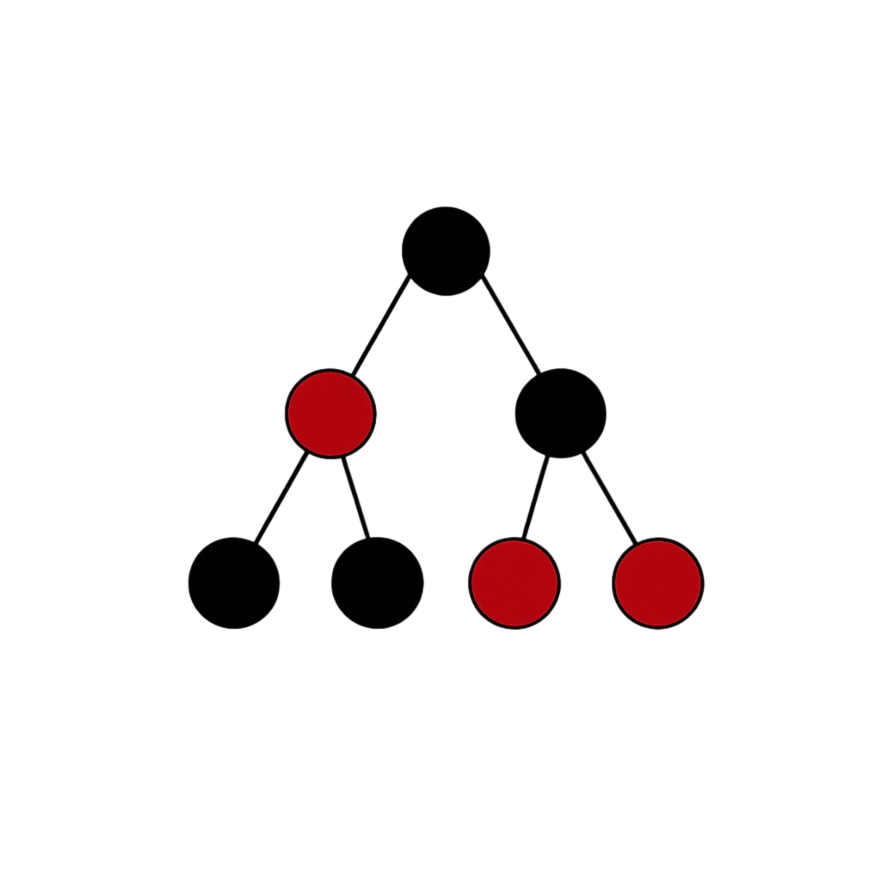
\includegraphics[height=0.55cm]{kcpc-logo.png}}}

\pagestyle{fancy}
\fancyhf{}
\lhead{\textcolor{kcpc-text}{\small\bfseries Problems}}
\rhead{\textcolor{kcpc-muted}{\small Week 2}}
\cfoot{\textcolor{kcpc-muted}{\small KCPC}}
\renewcommand{\headrulewidth}{0.4pt}
\renewcommand{\headrule}{\hbox
to\headwidth{\color{kcpc-red}\leaders\hrule height \headrulewidth\hfill}}
\renewcommand{\footrulewidth}{0pt}
\setlength{\headheight}{28pt}

\AddToShipoutPictureBG{%
    \begin{tikzpicture}[remember picture,overlay]
        \node[opacity=0.035, at=(current page.center)]
        {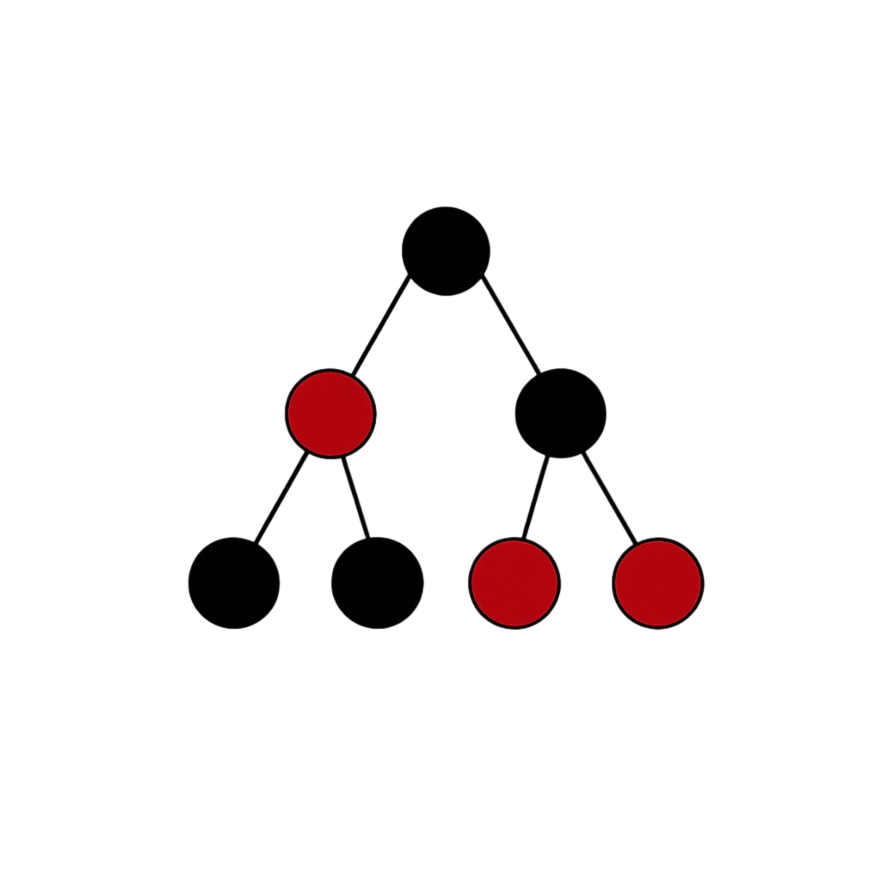
\includegraphics[width=0.38\paperwidth]{kcpc-logo.png}};
    \end{tikzpicture}%
}

\titleformat{\section}{\large\bfseries\color{kcpc-red}}{\thesection}{1em}{}

\setlist[itemize]{noitemsep, topsep=4pt}
\setlist[enumerate]{topsep=4pt}

\title{KCPC Week 2 Problems\\Advanced Invariants, Heuristics, and
Algorithmic Bridges}
\author{}
\date{}

\begin{document}
\maketitle
\thispagestyle{fancy}

\section*{How To Use This Sheet}
Each section builds on Week 1 techniques. Try the problems in order;
later ones generalise earlier ideas. For algorithmic bridge problems,
sketch the algorithm and argue correctness before writing code.

\section{Advanced Logic And Common Knowledge}

\subsection*{Basic -- Blue-Eyed Islanders ($k=2$)}
There are 2 islanders with blue eyes, and the rest have brown. They
cannot see their own eyes. A trusted outsider announces: ``At least
one of you has blue eyes.'' Each day, anyone who knows their own eye
colour leaves at midnight. What happens and on which day?

\subsection*{Easy -- Cheating Husbands}
In a village of 100 couples, some husbands have been unfaithful.
Every wife knows which \emph{other} husbands have cheated, but not
her own. The queen announces: ``At least one husband has been
unfaithful.'' If a wife deduces her husband cheated, she must act at
midnight. What happens?

\subsection*{Medium -- Sum And Product Puzzle}
Two integers $x,y$ with $2 \le x < y$ and $x+y \le 100$. Mr P knows
the product $xy$; Mr S knows the sum $x+y$.
P: ``I don't know the numbers.''
S: ``I knew you didn't know.''
P: ``Now I know the numbers.''
S: ``Now I know them too.''
Find $x$ and $y$.

\subsection*{Hard -- Cheryl's Birthday}
Cheryl gives Albert and Bernard a list of 10 possible dates. She
whispers the month to Albert and the day to Bernard.
Albert: ``I don't know the birthday, but I know Bernard doesn't know either.''
Bernard: ``At first I didn't know, but now I do.''
Albert: ``Now I also know.''
When is Cheryl's birthday?

\subsection*{Very Hard -- 100 Prisoners And A Light Bulb}
100 prisoners are in solitary cells. There is a central room with a
light bulb (initially off) and a switch. One prisoner at a time is
chosen randomly to visit the room; they may toggle the switch and/or
announce ``everyone has visited.'' If correct, all go free; if wrong,
all die. They may agree a strategy beforehand. Design a protocol that
guarantees freedom.

\section{Advanced Invariants And Monovariants}

\subsection*{Basic -- Peg Solitaire (Small Board)}
On a $3\times3$ board with the centre empty, pegs jump orthogonally
over adjacent pegs into empty squares, removing the jumped peg. Can
you finish with one peg in the centre?

\subsection*{Easy -- Token Game Modulo 3}
Tokens on integer points. A move: choose $x$ with tokens at $x$ and
$x+1$; remove them and place one at $x+2$. Start with one token at 0
and one at 1. Can you ever have a token at 100? (Hint: track $\sum
2^{\text{position}}$ modulo 3.)

\subsection*{Medium -- Conway's Soldiers}
On an infinite checkerboard, pegs occupy all squares with $y \le 0$.
A peg jumps orthogonally over another into an empty square, removing
the jumped peg. Can a peg ever reach $y=5$? (Hint: assign weights
$x^{|y|}$ with $x=(\sqrt{5}-1)/2$.)

\subsection*{Hard -- Polynomial Invariant For Grid Walks}
A token starts at $(0,0)$. A move changes $(x,y)$ to $(x+1,y+2)$ or
$(x+2,y+1)$. Characterise all reachable positions. (Hint: find a
polynomial $P(x,y)$ invariant under both moves.)

\subsection*{Very Hard -- IMO 1986 Problem 3 (Sequence Invariant)}
Given integer sequence $a_0, a_1, \ldots$ with $a_0 = 0$, $a_1 = 1$,
and $a_{n+1} = a_n + a_{n-1} + 1$. Prove that $a_n^2 -
a_{n-1}a_{n+1}$ is invariant modulo 3, and find its value.

\section{Colouring And Tiling: Generalisations}

\subsection*{Basic -- Tromino Tiling (Deficient Board)}
A $2^n \times 2^n$ board has one square removed. Prove it can be
tiled by L-shaped trominoes (three squares in an L). (Inductive construction.)

\subsection*{Easy -- Tiling With T-Tetrominoes}
Can a $4\times4$ board be tiled by T-tetrominoes (four squares in a T
shape)? Can a $4\times n$ board for $n>4$? Use a 4-colouring based on
coordinates mod 2.

\subsection*{Medium -- Fault-Free Domino Tiling}
A domino tiling of a rectangle has a fault line if a straight line
from one side to the other cuts no dominoes. Prove that a $6\times6$
board has a fault-free tiling, but a $6\times8$ board does not.

\subsection*{Hard -- Triominoes On A Chessboard}
Can an $8\times8$ chessboard with one corner removed be tiled by
straight trominoes ($1\times3$ rectangles)? Use a 3-colouring of the board.

\subsection*{Very Hard -- Generalised Mutilated Chessboard}
For which $m,n$ can an $m\times n$ board with two squares of opposite
colours removed be tiled by dominoes? Prove your characterisation.

\section{Induction And Recursion: From Proof To Algorithm}

\subsection*{Basic -- Josephus Problem}
$n$ people stand in a circle. Eliminate every second person until one
remains. Where should you stand to survive? Find a recurrence and
closed form for $J(n)$.

\subsection*{Easy -- Gray Codes}
An $n$-bit Gray code lists all $2^n$ binary strings so consecutive
strings differ in one bit. Give a recursive construction. Prove it
works by induction.

\subsection*{Medium -- Recursive 15-Puzzle Parity}
Given a $4\times4$ 15-puzzle configuration, design a recursive
algorithm to determine if it is solvable. Use the invariant from Week 1.

\subsection*{Hard -- Counterfeit Coin With $n$ Weighings}
Generalise the 12-coin, 3-weighing problem. With $n$ weighings on a
balance scale, what is the maximum number of coins among which you
can find one counterfeit (heavy or light)? Give a strategy achieving the bound.

\subsection*{Very Hard -- Hadamard Matrix Construction}
A Hadamard matrix of order $n$ is an $n\times n$ matrix with entries
$\pm1$ whose rows are mutually orthogonal. Give a recursive
construction for $n=2^k$ and prove it works.

\section{Zeitz Heuristics In Depth}

\subsection*{Basic -- Symmetry Strategy In Pairing Game}
Two players alternately place a domino on a $4\times4$ board.
Dominoes cannot overlap. The player who cannot move loses. Show the
second player has a winning strategy by symmetry.

\subsection*{Easy -- Extreme Principle For Points In A Circle}
Given 5 points in a unit circle, prove that some pair is at distance
$\le 1$. (Consider the extreme point farthest from the centre.)

\subsection*{Medium -- Wishful Thinking For A Number Puzzle}
Find all integer solutions to $x^2 + y^2 = 2z^2$ with $x,y,z > 0$.
(Wishful thinking: assume $x,y,z$ form a Pythagorean-like structure;
reduce to a known form.)

\subsection*{Hard -- Reduction To Graph Reachability}
$n$ lamps in a circle, each on or off. A move toggles lamp $i$ and
its two neighbours. From a given configuration, can you reach all
off? Model as a graph and use linear algebra over $\mathbb{F}_2$.

\subsection*{Very Hard -- Contest Problem: Combine Heuristics}
(From a past olympiad) A finite set of integers has the property that
for any two distinct elements, their sum is also in the set. Prove
the set is either $\{0\}$ or contains at least two elements whose sum
is 0. Use symmetry, extreme principle, and reduction.

\section{Algorithmic Bridges}

\subsection*{Basic -- Water Jugs As Graph Reachability}
Two jugs of capacities 3 and 5. Allowed: fill, empty, pour between
them. Model as a graph with states $(a,b)$. Use BFS conceptually to
find a sequence to measure exactly 4 units.

\subsection*{Easy -- Greedy Activity Selection}
You have $n$ intervals $[s_i, f_i]$. Choose a maximum-size subset of
non-overlapping intervals. Prove that picking the interval with
earliest finish time, then recursing, is optimal. (Exchange argument.)

\subsection*{Medium -- DP From Induction: Coin Change}
Given coin values $c_1, \ldots, c_k$ and target $n$, find the minimum
number of coins to make exactly $n$. Define $f(n)$ recursively,
identify overlapping subproblems, and give a tabulation algorithm.

\subsection*{Hard -- Sliding Puzzle State-Space Search}
$2\times3$ sliding puzzle with tiles 1--5 and one empty. From a given
start state, find the minimum moves to reach the goal. Describe the
state encoding, transitions, and why BFS works. (You may assume at
most 181,440 reachable states.)

\subsection*{Very Hard -- Greedy Scheduling With Deadlines}
$n$ jobs, each takes 1 unit of time, has a deadline $d_i$ and profit
$p_i$. You may schedule at most one job per time slot. A job only
earns profit if completed by its deadline. Design a greedy algorithm
to maximise total profit and prove it correct. (Hint: consider jobs
in decreasing profit order; use a disjoint-set union to find latest free slot.)

\end{document}
